Problemem w poprawnym opisie zależności między zmiennymi losowymi jest fakt, że dostępnych mamy wiele statystyk które ją mierzą. Każda z nich uchwyca pewien konkretny aspekt współzależności, i nie da się jasno wyróżnić konkretnej jako ,,najlepszej". W tej sekcji pracy zaprezentujemy wybrane narzędzia służące do badania struktury zależności zmiennych losowych.

\subsubsection{Współczynnik $\rho$ Pearsona}
Podstawową i najbardziej znaną miarą współzależności zmiennych losowych jest współczynnik korelacji liniowej Pearsona.

\begin{df}[Współczynnik korelacji liniowej Pearsona]
	Niech $X$ i $Y$ będą zmiennymi losowymi o skończonych drugich momentach. Współczynnikiem korelacji liniowej Pearsona $\rho$ nazywamy
	
	$$ \rho(X, Y) \coloneqq \Corr(X,Y) = \frac{\Cov(X,Y)}{\sqrt{\Var(X)}\sqrt{\Var(Y)}}.$$
\end{df}

Ten współczynnik korelacji przyjmuje wartości z zakresu $[-1, 1]$, gdzie $\vert\rho\vert=1$ oznacza idealną liniową relację. Jest on podstawową miarą zależności podawaną w każdym podręczniku do statystyki. Ma jednak szereg wad: nie jest zdefiniowany dla ciężkoogonowych rozkładów (przez nieokreśloną wariancję), nie zawiera pełnej informacji o strukturze zależności (poza przypadkiem wielowymiarowego rozkładu normalnego), oraz jest wrażliwy na monotonicznie rosnące przekształcenia $X$ i $Y$.\\

W rozdziale \ref{subsec:dwuwymiarowe_kopuly_probal} zauważymy, że jesteśmy w stanie zdefiniować miary współzależności, które nie będą brały pod uwagę rozkładów brzegowych zmiennych $X$ czy $Y$, lecz jedynie ich strukturę zależności (czyt. \cite{Scarsini1984}).

\subsubsection{Współczyniki $\tau$ Kendalla i $\rho$ Spearmana}

Współczynnikami należącymi do tej rodziny są $\tau$ Kendalla i $\rho$ Spearmana. Są one współczynnikami rangowymi, więc nie zależą od monotonicznych przekształceń rozkładów brzegowych $X$ czy $Y$. Dzięki temu mogą być jednoznacznie przedstawione w języku struktury zależności zmiennych losowych, co zazwyczaj nie jest możliwe dla współczynnika korelacji Pearsona.

\begin{df}[Współczynnik $\tau$ Kendalla]
	Współczynnik $\tau$ Kendalla między ciągłymi zmiennymi losowymi $X$ i $Y$ definiujemy jako:
	$$ \tau = \Pra[(X_1-X_2)(Y_1-Y_2)>0] - \Pra[(X_1-X_2)(Y_1-Y_2) <0], $$
	gdzie $(X_1, Y_1)$ i $(X_2, Y_2)$ są niezależnymi od siebie wektorami o tym samym rozkładzie co $(X, Y)$.
\end{df}

\begin{df}[Współczynnik $\rho$ Spearmana]
	Współczynnik $\rho$ Spearmana między ciągłymi zmiennymi losowymi $X$ i $Y$ o rozkładach brzegowych $F_X$ i $F_y$ zadany jest przez:
	$$ \rho = \Corr[F_X(X), F_Y(Y)].$$
\end{df}

Współczynniki te dają się jednoznacznie wyrazić za pomocą kopuł łączących $X$~i~$Y$~-~własność tę podamy w rozdziale \ref{subsec:dwuwymiarowe_kopuly_definicja}. Natomiast ich ekstremalne wartości, tj. $\vert\rho\vert=1$, czy $\vert\tau\vert=1$ implikują istotną w teorii kopuł własność współmonotoniczności lub przeciwmonotoniczności zmiennych losowych.

\subsubsection{Współmonotoniczność i przeciwmonotoniczność}
Współmonotoniczność i przeciwmonotoniczność to szczególne przypadki zależności zmiennych losowych, w których są one od siebie idealnie zależne.

\begin{df}[Zbiór współmonotoniczny]
	Zbiór $A \subset \R^2$ nazywamy współmonotonicznym, wtedy i tylko wtedy gdy dla dowolnych $(x_1, y_1)$, $(x_2, y_2)$ z $A$ zachodzi:
	
	$$ (x_1 - y_1)(x_2 - y_2) >0.$$
\end{df}

\begin{df}[Zbiór przeciwmonotoniczny]
	Zbiór $A \subset \R^2$ nazywamy przeciwmonotonicznym, wtedy i tylko wtedy gdy dla dowolnych $(x_1, y_1)$, $(x_2, y_2)$ z $A$ zachodzi:
	
	$$ (x_1 - y_1)(x_2 - y_2) <0.$$
\end{df}


\begin{df}[Zmienne losowe współ- i przeciwmonotoniczne]
	Wektor losowy $(X, Y)$ nazywamy współmonotonicznym (przeciwmonotonicznym) lub idealnie dodatnio (ujemnie) zależnym wtedy i tylko wtedy gdy istnieje zbiór współmonotoniczny (przeciwmonotoniczny) $A\subset\R^2$:
	
	$$ \Pra[(X,Y)\in A]=1.$$
\end{df}

Współmonotoniczność i przeciwmonotoniczność zmiennych losowych definiuje najsilniejszy rodzaj zależności jakie kopuły mogą reprezentować (czyt. twierdzenie \ref{thm:frechet_hoeffding}). Na ich podstawie można budować górne i dolne ograniczenia na siłę zależności zmiennych losowych, co z kolei pozwala np. na szacowanie górnych i dolnych ograniczeń cen opcji, czy miar ryzyka portfela aktywów (\cite{Cherubini_Copula_Methods_in_Finance}).

\subsubsection{Zależność ogonów}
Na zależność zmiennych losowych można popatrzeć również ze strony zależności obserwacji ekstremalnych. Rozważmy następującą statystykę:

\begin{df}[Współczynnik zależności ogonów]
	Górnym współczynnikiem zależności ogonów $(X_1, X_2)$ o rozkładach brzegowych $F_1$ i $F_2$ nazywamy:
	$$ \lambda^{u} = \lim\limits_{t\to1^{-}}\Pra[X_2 > F_2^{-1}(t) \vert X_1 > F_1^{-1}(t) ].$$
	Dolnym współczynnikiem nazywamy:
	$$ \lambda^{l} = \lim\limits_{t\to0^{+}}\Pra[X_2 \leqslant F_2^{-1}(t) \vert X_1 \leqslant F_1^{-1}(t) ].$$
\end{df}

Współczynniki zależności ogonów informują o sile zależności dwóch zmiennych losowych w sytuacjach gdy jedna z nich zaczyna przyjmować wartości ekstremalne. Mówimy, że zmienne losowe wykazują zależność ogonów jeśli $\lambda \in (0, 1]$ lub jej nie posiadają gdy $\lambda =0$. Te wspołczynniki zależą przede wszystkim od obserwacji będących ekstremalnymi względem obu zmiennych. Rysunek \ref{fig:tail_dependence} prezentuje przykładowy rozkład posiadający dolny współczynnik zależności ogonów, lecz nie posiadający górnego wspołczynnika. Kolorami zaznaczone są obserwacje które wpływają na dolny (szare punkty) i górny (czerwone punkty) współczynnik zależności ogonów.\\
W praktycznych zastosowaniach, jest on jednak trudny do kalibracji z danych - idea ta działa raczej w drugą stronę: z parametrów skalibrowanego modelu implikowany jest współczynnik zależności ogonów.
\begin{figure}[H]
	\centering
	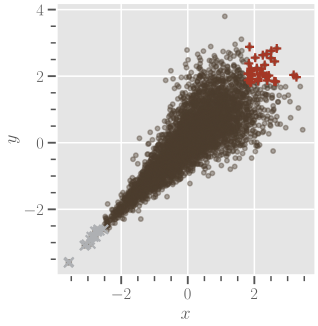
\includegraphics[width=0.5\linewidth]{01_Tail_dependence}	
	\caption{\textbf{Współczynnik zależności ogonów.} Rozkład o dolnym współczynniku i braku górnego współczynnika. Obserwacje zaznaczone na szaro wpływają na dolny współczynnik. Obserwacje zaznaczone na czerwono wpływają na górny współczynnik zależności ogonów.\label{fig:tail_dependence}}
\end{figure}

W tym rozdziale zdefiniowialiśmy różne miary pomagające nam zrozumieć zależność zmiennych losowych. Widzimy zatem, że korelacja Pearsona i modele eliptyczne to za mało, aby w pełni uchwycić charakter współzależności. W kolejnym rozdziale podamy teorię \emph{kopuł}, które dadzą nam odpowiednie narzędzia do rozwiązania tego problemu.